\section{Abstract Factory}

O padrão Abstract Factory define uma família 
de objetos relacionados e uma interface para 
criá-los, sem definir a implementação. Dessa 
forma, diferentes implementações desse 
conjunto de objetos podem ser utilizadas 
sem que as classes cliente que os utilizam 
precisem conhecer sua implementação.

O diagrama apresentado na figura \ref{abfactory_struct} 
demonstra a estrutura desse padrão, onde a 
interface AbstractFactory suporta as famílias 
ConcreteFactory1 e ConcreteFactory2, com cada uma 
delas definindo qual implementação das interfaces 
AbstractProductA e AbstractProductB serão 
utilizadas.

\begin{figure}[htb]
	\caption{\label{abfactory_struct}Estrutura do Abstract Factory}
	\begin{center}
	    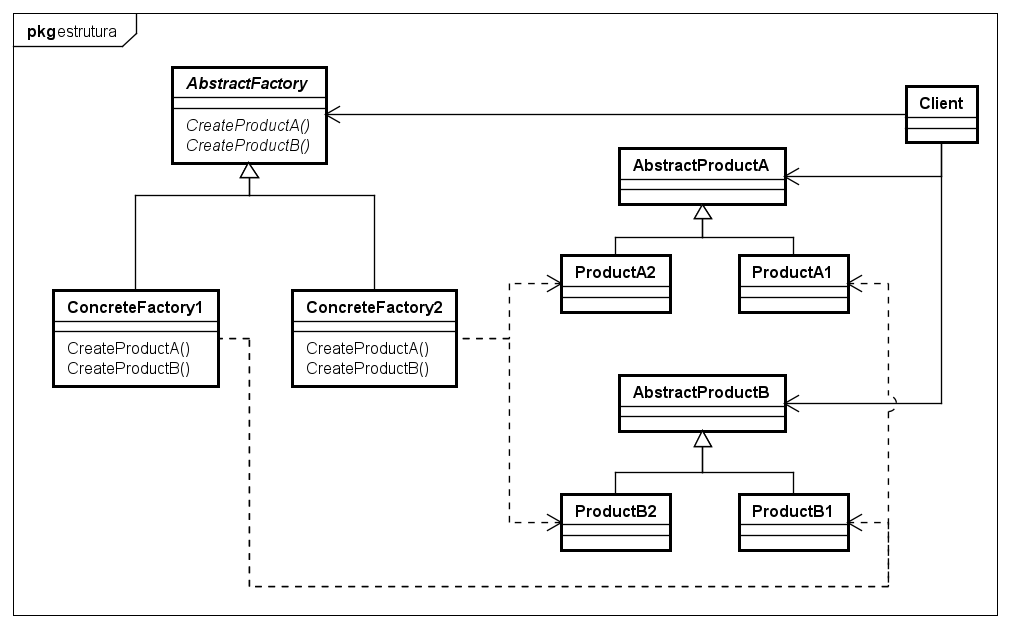
\includegraphics[scale=0.5]{5_padroes-contexto-funcional/5.1_criacionais/5.1.2_abstract-factory/abstractfactory_estrutura.png}
	\end{center}
\end{figure}

\subsection*{Exemplo Orientado a Objetos}

Como exemplo, é apresentado um \textit{toolkit} 
que suporta tipos diferentes de interação para 
seus \textit{widgets}, como Motif ou Presentation 
Maneger (PM). Dessa forma, para que a aplicação 
não precise ser dependente de cada tipo 
diferente de \textit{widgets}, é 
utilizado o padrão Abstract Factory para 
definir uma família de objetos de Widget 
diferente para cada tipo de interação. 

A implementação do padrão é demonstrada no 
diagrama de classes da figura \ref{abfactory_exemplo} 
e no código \ref{ooabfactory}. Uma interface 
WidgetFactory define as operações de criação 
de todos os \textit{widgets} possíveis, enquanto 
as classes MotifWidgetFactory e PMWidgetFactory 
implementam sua criação para os tipos de 
interação suportados.

\begin{figure}[htb]
	\caption{\label{abfactory_exemplo}Exemplo de Abstract Factory}
	\begin{center}
	    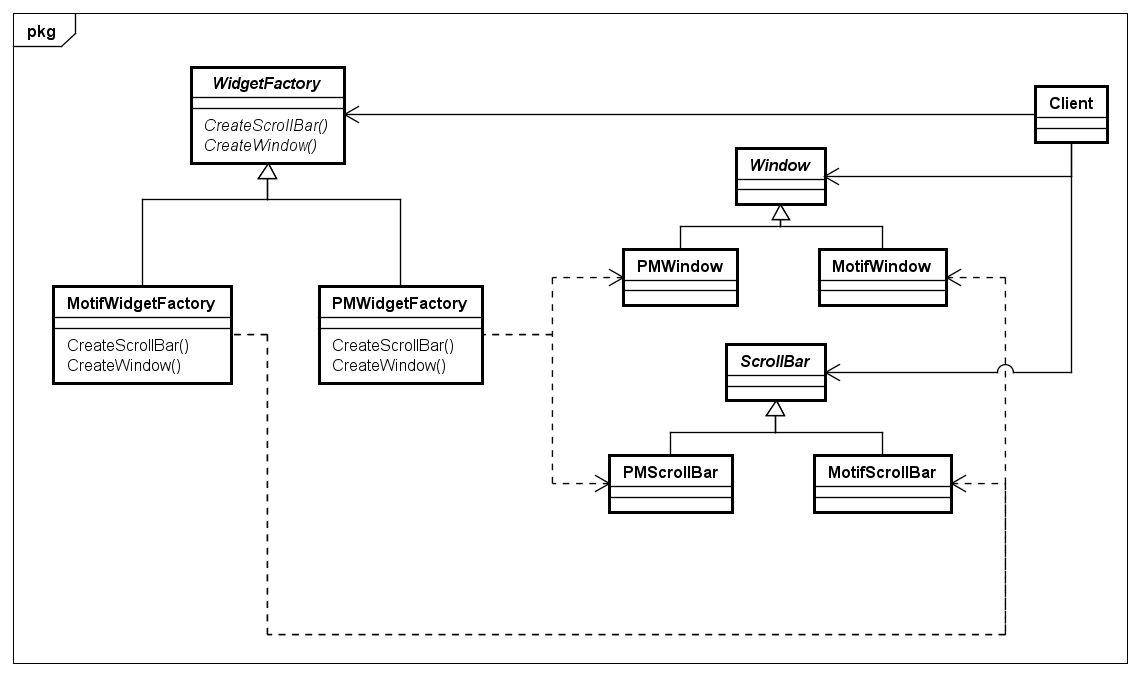
\includegraphics[scale=0.5]{5_padroes-contexto-funcional/5.1_criacionais/5.1.2_abstract-factory/abstractfactory_exemplo.png}
	\end{center}
\end{figure}

\begin{lstlisting}[caption={Abstract Factory Orientado a Objetos},label=ooabfactory]
	
trait WidgetFactory {
  def CreateScrollBar() : ScrollBar
  def CreateWindow() : Window
}

trait Window 
trait ScrollBar

class MotifWidgetFactory extends WidgetFactory {
  def CreateScrollBar(): ScrollBar = new MotifScrollBar()
  def CreateWindow(): Window = new MotifWindow()
}

class PMWidgetFactory extends WidgetFactory {
  def CreateWindow(): Window = new PMWindow()
  def CreateScrollBar(): ScrollBar = new PMScrollBar()
}

class PMWindow extends Window {
  // Implementação de PMWindow
}

class MotifWindow extends Window {
  // Implementação de MotifWindow
}

class PMScrollBar extends ScrollBar {
  // Implementação de PMScrollBar
}

class MotifScrollBar extends ScrollBar {
  // Implementação de MotifScrollBar
}

\end{lstlisting}



\subsection*{Contexto Funcional}

\begin{lstlisting}[caption={Abstract Factory Funcional},label=fpabfactory]
    
    

\end{lstlisting}